\begin{figure}
    \centering
    \caption{Size k=3 cache vs k=4 cache in stack algorithm }
    \label{fig:my_label}
\begin{tikzpicture}


    \node[rounded corners,draw=black,label=above:K, minimum size=2cm] (a) at (0,0)  {
    \begin{tikzpicture}
        \node[rounded corners,draw=black,minimum size=0.8cm]{a};
    \end{tikzpicture}
    
\begin{tikzpicture}
        \node[rounded corners,draw=black,minimum size=0.8cm]{};
    \end{tikzpicture}
    
\begin{tikzpicture}
        \node[rounded corners,draw=black,minimum size=0.8cm]{};
    \end{tikzpicture}
    };
    \node[text width=3cm] at (-3, 0) 
    {Cold start miss, a added to cache};

    
    \node[rounded corners,draw=black,minimum size=2cm] (b) at (0,-2.5)  {   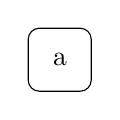
\begin{tikzpicture}
        \node[rounded corners,draw=black,minimum size=0.8cm]{a};
    \end{tikzpicture}
    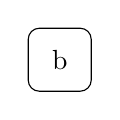
\begin{tikzpicture}
        \node[rounded corners,draw=black,minimum size=0.8cm]{b};
    \end{tikzpicture}
    
\begin{tikzpicture}
        \node[rounded corners,draw=black,minimum size=0.8cm]{};
    \end{tikzpicture}
    };
     \node[text width=3cm] at (-3,-2.5) 
    {Cold start miss, b added to cache};

    
    \node[rounded corners,draw=black,minimum size=2cm] (c) at (0,-5)  {   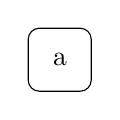
\begin{tikzpicture}
        \node[rounded corners,draw=black,minimum size=0.8cm]{a};
    \end{tikzpicture}
    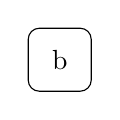
\begin{tikzpicture}
        \node[rounded corners,draw=black,minimum size=0.8cm]{b};
    \end{tikzpicture}
    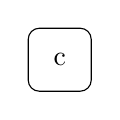
\begin{tikzpicture}
        \node[rounded corners,draw=black,minimum size=0.8cm]{c};
    \end{tikzpicture}
    };
    \node[text width=3cm] at (-3,-5) 
    {Cold start miss, c added to cache};

      
    \node[rounded corners,draw=black,minimum size=2cm] (d) at (0,-7.5)  {   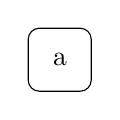
\begin{tikzpicture}
        \node[rounded corners,draw=black,minimum size=0.8cm]{a};
    \end{tikzpicture}
    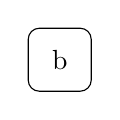
\begin{tikzpicture}
        \node[rounded corners,draw=black,minimum size=0.8cm]{b};
    \end{tikzpicture}
    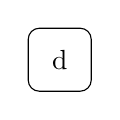
\begin{tikzpicture}
        \node[rounded corners,draw=black,minimum size=0.8cm]{d};
    \end{tikzpicture}
    };

     \node[text width=3cm] at (-3,-7.5) 
    {Cold start miss, D added to cache, evict C since FITF};

    
    \node[rounded corners,draw=black,minimum size=2cm, below left=1 cm of d] (e) at (2.2,-8.4)  { 
    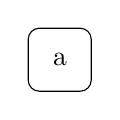
\begin{tikzpicture}
        \node[rounded corners,draw=black,minimum size=0.8cm]{a};
    \end{tikzpicture}
    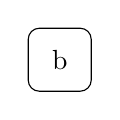
\begin{tikzpicture}
        \node[rounded corners,draw=black,minimum size=0.8cm]{b};
    \end{tikzpicture}
    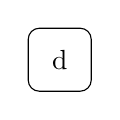
\begin{tikzpicture}
        \node[rounded corners,draw=black,minimum size=0.8cm]{d};
    \end{tikzpicture}
    };  

     \node[text width=3cm] at (-2.5,-9.8) 
    {Hit on A};
    
    \node[rounded corners,draw=black,minimum size=2cm,below left=1 cm of e] (f) at (2.2,-10.8)  { 
    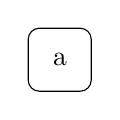
\begin{tikzpicture}
        \node[rounded corners,draw=black,minimum size=0.8cm]{a};
    \end{tikzpicture}
    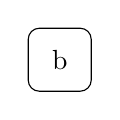
\begin{tikzpicture}
        \node[rounded corners,draw=black,minimum size=0.8cm]{b};
    \end{tikzpicture}
    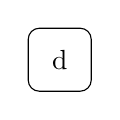
\begin{tikzpicture}
        \node[rounded corners,draw=black,minimum size=0.8cm]{d};
    \end{tikzpicture}
    };  

     \node[text width=3cm] at (-2.5,-12.2) 
    {Hit on B};

    
    \node[rounded corners,draw=black,minimum size=2cm, below left=1 cm of f] (g) at (2.2,-13.4)  { 
    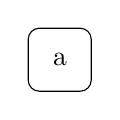
\begin{tikzpicture}
        \node[rounded corners,draw=black,minimum size=0.8cm]{a};
    \end{tikzpicture}
    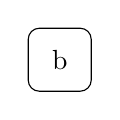
\begin{tikzpicture}
        \node[rounded corners,draw=black,minimum size=0.8cm]{b};
    \end{tikzpicture}
    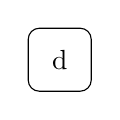
\begin{tikzpicture}
        \node[rounded corners,draw=black,minimum size=0.8cm]{d};
    \end{tikzpicture}
    };  

     \node[text width=3cm] at (-3,-14.7) 
    {Capacity miss C, evict D};
    
    \node[rounded corners,draw=black,minimum size=2cm, below left=1 cm of g] (h) at (2.2,-15.6)  { 
    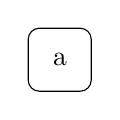
\begin{tikzpicture}
        \node[rounded corners,draw=black,minimum size=0.8cm]{a};
    \end{tikzpicture}
    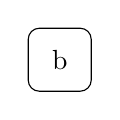
\begin{tikzpicture}
        \node[rounded corners,draw=black,minimum size=0.8cm]{b};
    \end{tikzpicture}
    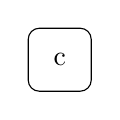
\begin{tikzpicture}
        \node[rounded corners,draw=black,minimum size=0.8cm]{c};
    \end{tikzpicture}
    }; 
    \node[text width=3cm] at (-2.5,-17.3) 
    {Hit on C};
     \node[rounded corners,draw=black,label=above:k+1, minimum size=2cm] (i) at (6,0)  {
    
\begin{tikzpicture}
        \node[rounded corners,draw=black,minimum size=0.8cm]{};
    \end{tikzpicture}
    
\begin{tikzpicture}
        \node[rounded corners,draw=black,minimum size=0.8cm]{};
    \end{tikzpicture}
    
\begin{tikzpicture}
        \node[rounded corners,draw=black,minimum size=0.8cm]{};
    \end{tikzpicture}
    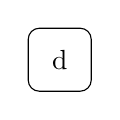
\begin{tikzpicture}
        \node[rounded corners,draw=black,minimum size=0.8cm]{d};
    \end{tikzpicture}
    };
    
    \node[rounded corners,draw=black,minimum size=2cm] (j) at (6,-2.5)  {   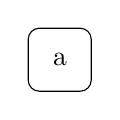
\begin{tikzpicture}
        \node[rounded corners,draw=black,minimum size=0.8cm]{a};
    \end{tikzpicture}
    
\begin{tikzpicture}
        \node[rounded corners,draw=black,minimum size=0.8cm]{};
    \end{tikzpicture}
    
\begin{tikzpicture}
        \node[rounded corners,draw=black,minimum size=0.8cm]{};
    \end{tikzpicture}
    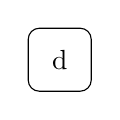
\begin{tikzpicture}
        \node[rounded corners,draw=black,minimum size=0.8cm]{d};
    \end{tikzpicture}
    };
    
    \node[rounded corners,draw=black,minimum size=2cm] (k) at (6,-5)  {   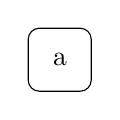
\begin{tikzpicture}
        \node[rounded corners,draw=black,minimum size=0.8cm]{a};
    \end{tikzpicture}
    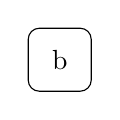
\begin{tikzpicture}
        \node[rounded corners,draw=black,minimum size=0.8cm]{b};
    \end{tikzpicture}
    
\begin{tikzpicture}
        \node[rounded corners,draw=black,minimum size=0.8cm]{};
    \end{tikzpicture}
    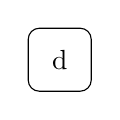
\begin{tikzpicture}
        \node[rounded corners,draw=black,minimum size=0.8cm]{d};
    \end{tikzpicture}
    };

      
    \node[rounded corners,draw=black,minimum size=2cm] (l) at (6,-7.5)  {   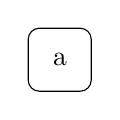
\begin{tikzpicture}
        \node[rounded corners,draw=black,minimum size=0.8cm]{a};
    \end{tikzpicture}
    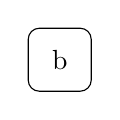
\begin{tikzpicture}
        \node[rounded corners,draw=black,minimum size=0.8cm]{b};
    \end{tikzpicture}
    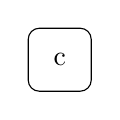
\begin{tikzpicture}
        \node[rounded corners,draw=black,minimum size=0.8cm]{c};
    \end{tikzpicture}
    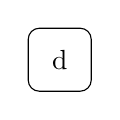
\begin{tikzpicture}
        \node[rounded corners,draw=black,minimum size=0.8cm]{d};
    \end{tikzpicture}
    };
    
    \node[rounded corners,draw=black,minimum size=2cm, below left=1 cm of l] (m) at (8.7,-8.4)  { 
    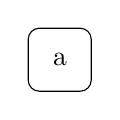
\begin{tikzpicture}
        \node[rounded corners,draw=black,minimum size=0.8cm]{a};
    \end{tikzpicture}
    
\begin{tikzpicture}
        \node[rounded corners,draw=black,minimum size=0.8cm]{??};
    \end{tikzpicture}
    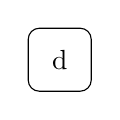
\begin{tikzpicture}
        \node[rounded corners,draw=black,minimum size=0.8cm]{d};
    \end{tikzpicture}
    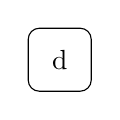
\begin{tikzpicture}
        \node[rounded corners,draw=black,minimum size=0.8cm]{d};
    \end{tikzpicture}
    };  
    \node[rounded corners,draw=black,minimum size=2cm,below left=1 cm of m] (n) at (8.7,-10.8)  { 
    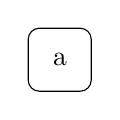
\begin{tikzpicture}
        \node[rounded corners,draw=black,minimum size=0.8cm]{a};
    \end{tikzpicture}
    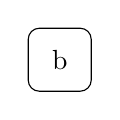
\begin{tikzpicture}
        \node[rounded corners,draw=black,minimum size=0.8cm]{b};
    \end{tikzpicture}
    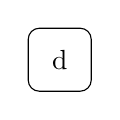
\begin{tikzpicture}
        \node[rounded corners,draw=black,minimum size=0.8cm]{d};
    \end{tikzpicture}
    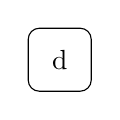
\begin{tikzpicture}
        \node[rounded corners,draw=black,minimum size=0.8cm]{d};
    \end{tikzpicture}
    };  
    \node[rounded corners,draw=black,minimum size=2cm, below left=1 cm of n] (o) at (8.7,-13.4)  { 
    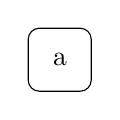
\begin{tikzpicture}
        \node[rounded corners,draw=black,minimum size=0.8cm]{a};
    \end{tikzpicture}
    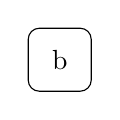
\begin{tikzpicture}
        \node[rounded corners,draw=black,minimum size=0.8cm]{b};
    \end{tikzpicture}
    \begin{tikzpicture}
        \node[rounded corners,draw=black,minimum size=0.8cm]{d};
    \end{tikzpicture}
    \begin{tikzpicture}
        \node[rounded corners,draw=black,minimum size=0.8cm]{d};
    \end{tikzpicture}
    };  
    \node[rounded corners,draw=black,minimum size=2cm, below left=1 cm of o] (p) at (8.7,-15.9)  { 
    \begin{tikzpicture}
        \node[rounded corners,draw=black,minimum size=0.8cm]{a};
    \end{tikzpicture}
    \begin{tikzpicture}
        \node[rounded corners,draw=black,minimum size=0.8cm]{b};
    \end{tikzpicture}
    \begin{tikzpicture}
        \node[rounded corners,draw=black,minimum size=0.8cm]{d};
    \end{tikzpicture}
    \begin{tikzpicture}
        \node[rounded corners,draw=black,minimum size=0.8cm]{d};
    \end{tikzpicture}
    };  
                
    \draw[thick,->] (i) -- (j);
    \draw[thick,->](j) -- (k);  
    \draw[thick,->](k) -- (l);  
    \draw[thick,->](l) -- (m);  
    \draw[thick,->] (m) -- (n);
    \draw[thick,->](n) -- (o);  
    \draw[thick,->](o) -- (p);
\end{tikzpicture}
\end{figure}